\documentclass{report}
% Ćirilica: kodiranje fonta i jezik (srpski, ćirilica)
\usepackage[T2A]{fontenc}
\usepackage[utf8]{inputenc}
\usepackage[serbianc]{babel}

% Veličina strane i margine
\usepackage[a4paper,top=2cm,bottom=2cm,left=2.5cm,right=2.5cm]{geometry}

% Korisni paketi
\usepackage{amsmath}
\usepackage{graphicx}
\usepackage{float}
\usepackage{multirow}
\usepackage{array}
\usepackage{enumitem}
\usepackage{tcolorbox}
\tcbuselibrary{skins,breakable}
\usepackage[colorlinks=true, allcolors=blue]{hyperref}

% Главе без нове стране и без великог размака, да се текст лепо пакује
\usepackage{titlesec}
\titleclass{\chapter}{straight}
\titleformat{\chapter}{\normalfont\LARGE\bfseries}{\thechapter.}{0.5em}{}
\titlespacing*{\chapter}{0pt}{18pt}{10pt}

\setcounter{secnumdepth}{2}
\setcounter{tocdepth}{1}

% Мање празнине око слика
\setlength{\textfloatsep}{10pt plus 2pt minus 2pt}
\setlength{\intextsep}{10pt plus 2pt minus 2pt}

% Оквир за кључне податке
\newtcolorbox{kljucno}{breakable, colback=blue!4, colframe=blue!45!black,
    boxrule=0.5pt, arc=1.5pt, left=6pt, right=6pt, top=3pt, bottom=3pt}

% Оквир за поделе: ужи, центриран, наслов на ивици оквира
\newtcolorbox{podela}[1]{enhanced, width=0.8\linewidth, center,
    colback=green!3, colframe=green!45!black, boxrule=0.6pt, arc=2pt,
    title={#1}, fonttitle=\bfseries\small, coltitle=white,
    colbacktitle=green!45!black,
    attach boxed title to top left={xshift=4mm, yshift=-2.2mm},
    boxed title style={boxrule=0pt, arc=1pt},
    top=4mm, bottom=2mm, left=2mm, right=2mm, fontupper=\small,
    before skip=8pt, after skip=8pt}

% Нумерисана листа унутар подела
\newlist{lista}{enumerate}{2}
\setlist[lista,1]{label=\arabic*., noitemsep, topsep=0pt, leftmargin=1.6em}
\setlist[lista,2]{label=\alph*), noitemsep, topsep=0pt, leftmargin=1.4em}

% Већа слика (шеме): до 9 cm висока
\newcommand{\slikaV}[4][0.7]{%
\begin{figure}[!htb]
    \centering
    \IfFileExists{slike/#2}%
        {\includegraphics[width=#1\textwidth,height=9cm,keepaspectratio]{slike/#2}}%
        {\fbox{\parbox[c][4cm][c]{#1\textwidth}{\centering\small слика: \texttt{slike/#2}}}}
    \caption{#3}
    \label{#4}
\end{figure}}

% Слика: мала, највише 5 cm висока, плута да не оставља празна места
%   [#1] ширина (део ширине текста), #2 фајл у фолдеру slike, #3 натпис, #4 ознака
\newcommand{\slika}[4][0.45]{%
\begin{figure}[!htb]
    \centering
    \IfFileExists{slike/#2}%
        {\includegraphics[width=#1\textwidth,height=5cm,keepaspectratio]{slike/#2}}%
        {\fbox{\parbox[c][2.5cm][c]{#1\textwidth}{\centering\small слика: \texttt{slike/#2}}}}
    \caption{#3}
    \label{#4}
\end{figure}}

\title{Аутоелектронски системи 2 -- Осветљење и сигнализација}
\author{Саобраћајно техничка школа, Београд, Земун}
\date{}

\begin{document}
\maketitle
\tableofcontents
\newpage

%##################################################################
\chapter{Осветљење и сигнализација}
%##################################################################

Светлосна и сигнална опрема возила одређена је међународним и националним
прописима, а њена исправност проверава се на сваком техничком прегледу.

\begin{kljucno}
\centering\textbf{Возач мора добро да види и да буде добро виђен.}
\end{kljucno}

Фарови осветљавају пут и служе за упозоравање (блинкање), мигавци најављују
промену правца, а сва четири мигавца упозоравају на опасност.

\section{Светлосна опрема возила}

\begin{podela}{Подела светлосне опреме}
\begin{lista}
    \item По намени:
    \begin{lista}
        \item опрема за осветљавање (фарови),
        \item сигнална опрема (мигавци, стоп, позициона и остала светла).
    \end{lista}
    \item По положају:
    \begin{lista}
        \item на предњој страни возила,
        \item на задњој страни возила,
        \item у унутрашњости возила.
    \end{lista}
\end{lista}
\end{podela}

\begin{minipage}[t]{0.48\linewidth}
\textbf{Напред:}
\begin{itemize}[noitemsep, topsep=2pt, leftmargin=1.2em]
    \item фарови за дуга и оборена светла,
    \item фарови за маглу,
    \item додатни фарови за дуга светла,
    \item мигавци,
    \item паркирна светла,
    \item позициона и габаритна светла,
    \item дневна светла.
\end{itemize}
\end{minipage}\hfill
\begin{minipage}[t]{0.48\linewidth}
\textbf{Позади:}
\begin{itemize}[noitemsep, topsep=2pt, leftmargin=1.2em]
    \item стоп-светла,
    \item позициона светла,
    \item светло за маглу (црвено),
    \item мигавци,
    \item паркирна и габаритна светла,
    \item светла за вожњу уназад (бела),
    \item светло регистарске таблице.
\end{itemize}
\end{minipage}

\medskip
У \textbf{унутрашњости} се осветљавају инструменти, прекидачи, кабина и
пртљажник, а светлосни и звучни сигнали упозоравају возача на кварове.

\section{Прописи и ознаке}

Опрема која је испитана и одобрена носи утиснуту ознаку:

\begin{podela}{Ознаке одобрења}
\begin{lista}
    \item \textbf{E} -- ECE правилници (цела Европа),
    \item \textbf{e} -- прописи Европске уније,
    \item посебна ознака -- немачки национални стандард.
\end{lista}
\end{podela}

У Америци произвођачи сами издају сертификате. Наши стандарди заснивају се на
немачким DIN стандардима и усклађују се са европским.

\section{Оптичка опажања}

Око се прилагођава светлу мењањем величине зенице и осетљивости мрежњаче.
Возач око 90\,\% информација прима видом.

\begin{kljucno}
Око је најосетљивије на жуто-зелену светлост ($\lambda = 555$~nm). Видљива
светлост је од 380 до 780~nm; UV и IR зрачење око не види.
\end{kljucno}

\textbf{Даљина видљивости} је највеће растојање на коме се објекат на путу
још уочава. Зависи од објекта, подлоге и чистоће фара: на сувом коловозу може
бити преко 100~m, а на мокром испод 20~m.

%##################################################################
\chapter{Светлосни извори -- сијалице}
%##################################################################

Загрејана тела зраче светлост, али само мали део енергије постаје светлост, а
већина топлота. Зато класичне сијалице имају мали степен искоришћења (испод
10\,\%) и потискују их новије врсте.

\begin{podela}{Подела светлосних извора}
\begin{lista}
    \item сијалице са ужареним влакном (и Bilux),
    \item халогене сијалице,
    \item гасне (ксенонске) сијалице,
    \item LED диоде.
\end{lista}
\end{podela}

\section{Сијалице са ужареним влакном}

\textbf{Волфрамово влакно} налази се у стакленом балону из ког је извучен
ваздух. Један крај влакна везан је за подножје (маса), а други за изоловани
прикључак. Што је влакно топлије, светли јаче, али волфрам брже испарава и
таложи се на стаклу, па балон тамни, а влакно се тањи. Сијалице веће снаге
пуне се инертним гасом, који смањује испаравање. Поцрнелу сијалицу треба
заменити и ако није прегорела.

\begin{kljucno}
Напон већи за 10\,\% даје 45\,\% више светлости, али скраћује век сијалице на
мање од трећине.
\end{kljucno}

\begin{podela}{Предности сијалица са ужареним влакном}
\begin{lista}
    \item једноставне и јефтине,
    \item раде директно на напону акумулатора, без електронике,
    \item одмах светле пуном јачином,
    \item лако се мењају.
\end{lista}
\end{podela}

\textbf{Данас} се користе углавном за сигнална светла (мигавци, стоп,
позициона светла, светло таблице) и унутрашње осветљење, као и код
старијих возила. Све више их замењују LED диоде.

\paragraph*{Bilux сијалица} има \textbf{два влакна}, која никад не светле
истовремено:
\begin{itemize}[noitemsep]
    \item влакно за \textbf{дуго светло} -- у жижи рефлектора, попречно,
    \item влакно за \textbf{оборено светло} -- испред жиже, уздужно, са
          металним \textbf{заклоном} испод, који не пушта светлост на доњи
          део рефлектора.
\end{itemize}
Ако је једна страна заклона закошена за $15^\circ$, оборено светло је
\textbf{асиметрично} (десна ивица пута осветљена је даље).

\section{Халогене сијалице}

Влакно је у цевчици од \textbf{кварцног стакла}, напуњеној инертним гасом са
малом количином \textbf{јода или брома}.

\textbf{Халогени кружни процес:} испарени волфрам се у хладнијем делу цевчице
(200--1400\,$^\circ$C) једини са халогеним гасом. Једињење се не таложи на
стаклу, већ се враћа ка влакну и на око 3400\,$^\circ$C распада: волфрам се
враћа на влакно, а халоген креће у нови круг. Зато стакло не тамни, а век је
дужи. Зид цевчице мора бити топао (око 300\,$^\circ$C), па је цевчица мала.

\begin{kljucno}
Халогену сијалицу \textbf{не смемо дирати прстима} -- масне мрље на врелом
стаклу оштећују цевчицу.
\end{kljucno}

\begin{podela}{Предности халогених сијалица}
\begin{lista}
    \item јаче светло од класичних сијалица исте снаге,
    \item дужи век трајања,
    \item стакло не тамни, па светло не слаби током века,
    \item одмах светле пуном јачином, без уређаја за паљење,
    \item знатно јефтиније од гасних и LED фарова.
\end{lista}
\end{podela}

\textbf{Данас} су и даље веома распрострањене у фаровима за дуго и оборено
светло (H4, H7) и у фаровима за маглу, нарочито код јефтинијих и старијих
возила.

\section{Гасне сијалице}

Раде на принципу \textbf{електричног пражњења у гасу} (ксенон и метални
халогениди). Уређај за паљење даје \textbf{10--20~kV}, гас се јонизује и пали
се \textbf{електрични лук}, а затим сијалица ради на наизменичној струји од
око 400~Hz. У аутомобилима се користе у систему \textbf{LITRONIC}.

\begin{podela}{Предности гасних сијалица}
\begin{lista}
    \item дуг век (нема влакна које се троши),
    \item светлост ближа дневној (преко 4000~K),
    \item већи степен искоришћења уз мању потрошњу.
\end{lista}
\end{podela}

\textbf{Данас} их у новим возилима потискују LED фарови, али их има у великом
броју возила произведених од краја деведесетих до средине 2010-их.

\section{Сијалице за моторна возила}

Праве се за напоне \textbf{6, 12 и 24~V}, са различитим подножјима, да се не
би замениле, и са утиснутом ознаком
(слике~\ref{fig:sijalice1}--\ref{fig:sijalice3}).

\begin{figure}[H]
    \centering
    % --- gornji red: dve slike ---
    \begin{minipage}{0.48\textwidth}
        \centering
        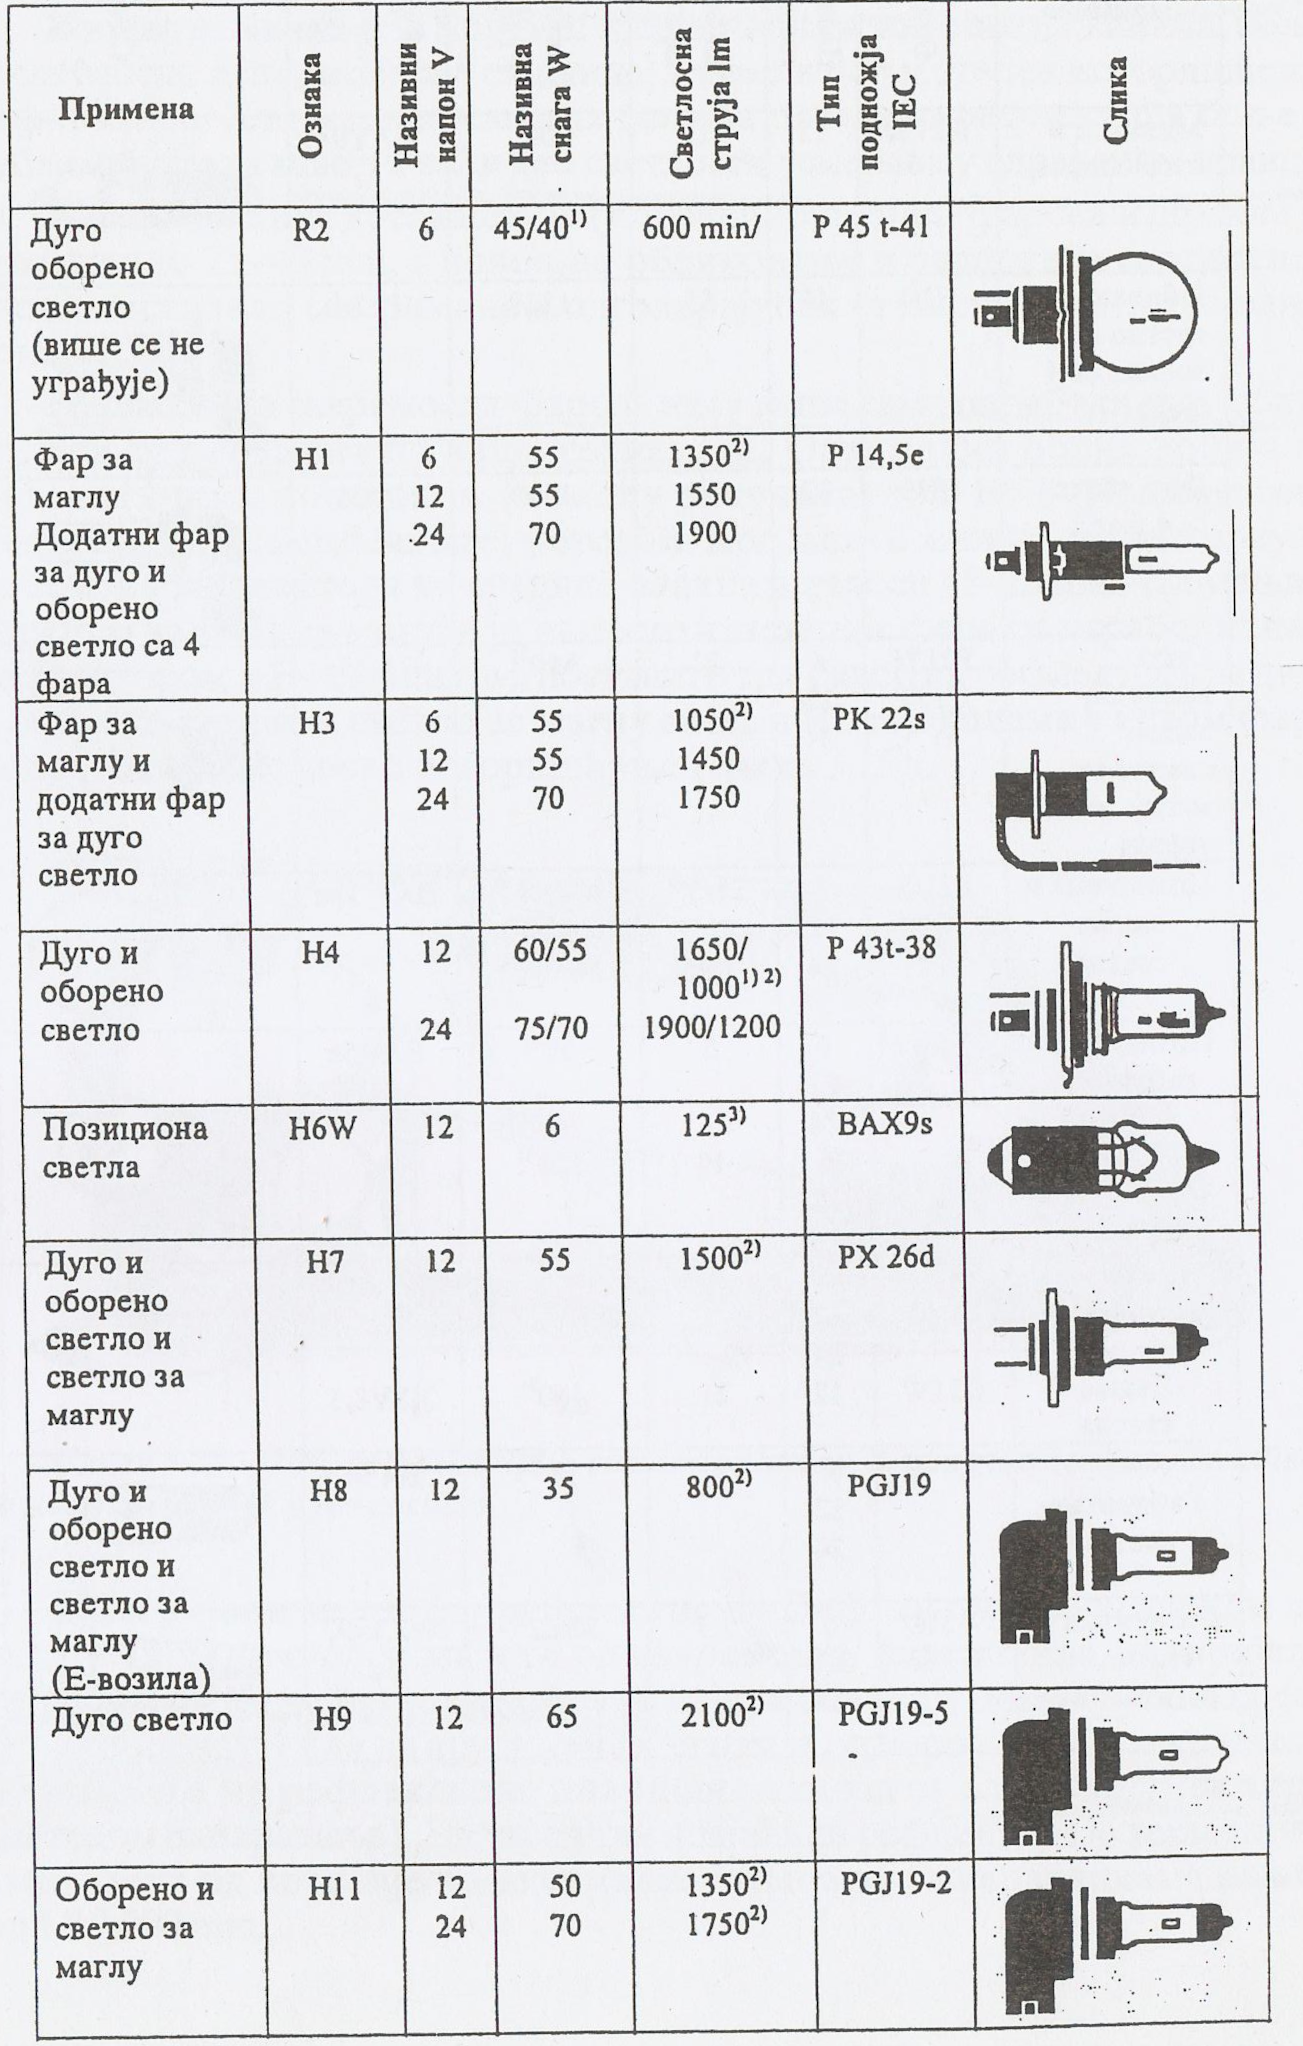
\includegraphics[width=\linewidth]{slike/sijalice1.png}
        \caption{Сијалица ...} % TODO: натпис
        \label{fig:sijalice1}
    \end{minipage}
    \hfill
    \begin{minipage}{0.48\textwidth}
        \centering
        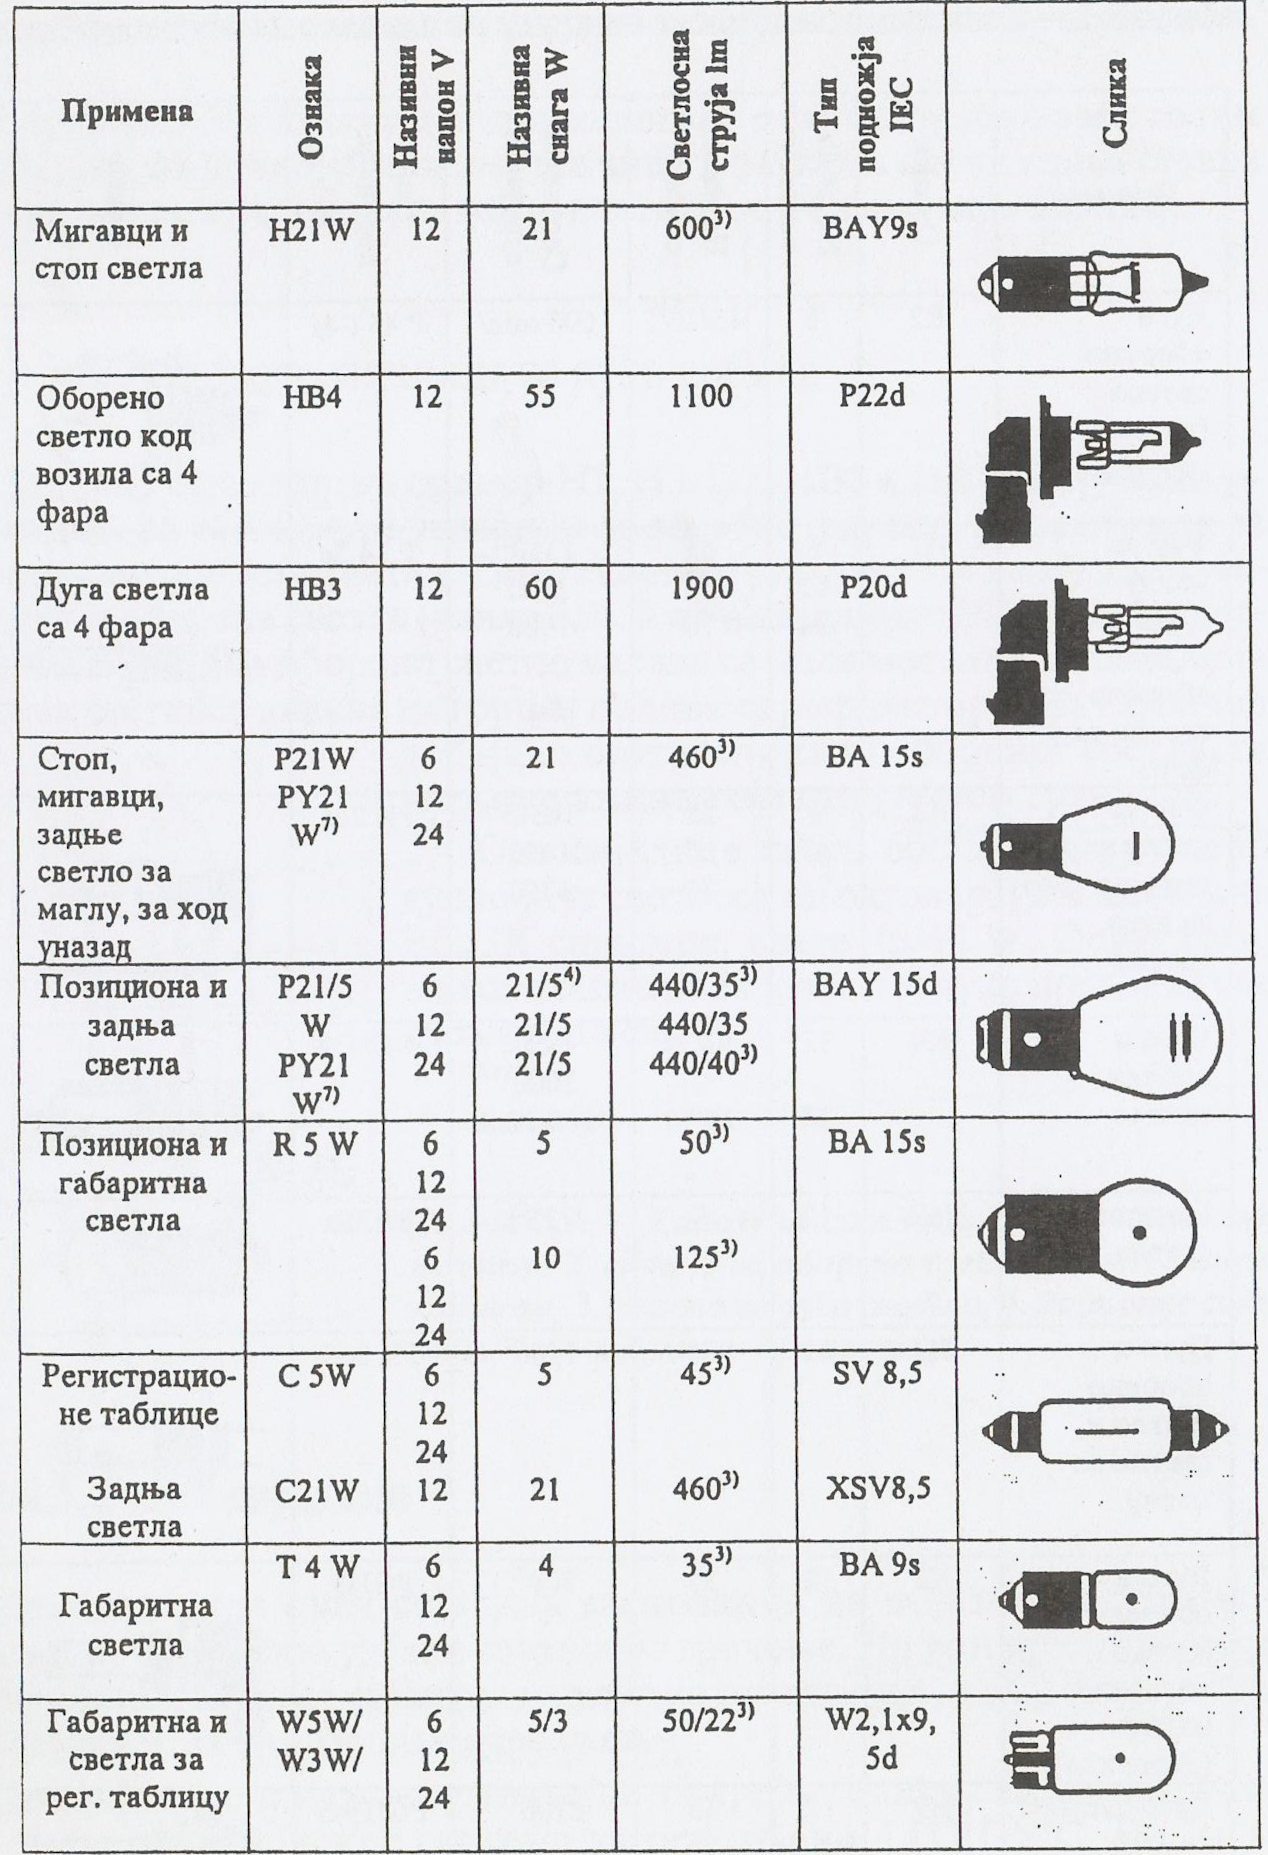
\includegraphics[width=\linewidth]{slike/sijalice2.png}
        \caption{Сијалица ...} % TODO: натпис
        \label{fig:sijalice2}
    \end{minipage}

    \vspace{0.5cm}

    % --- donji red: treća slika ---
    \begin{minipage}{0.6\textwidth}
        \centering
        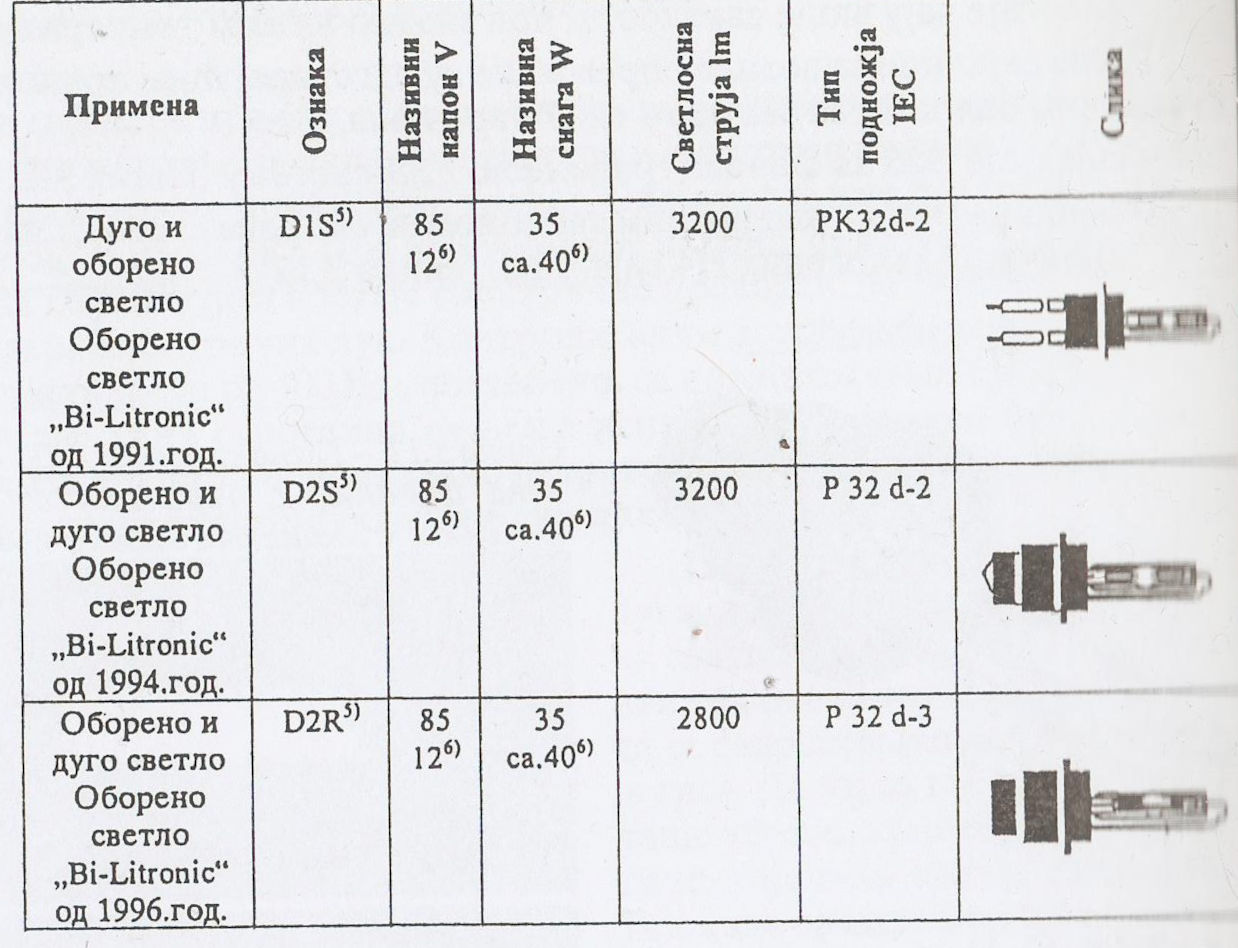
\includegraphics[width=\linewidth]{slike/sijalice3.png}
        \caption{Сијалица ...} % TODO: натпис
        \label{fig:sijalice3}
    \end{minipage}
\end{figure}

\begin{podela}{Светлосне величине}
\begin{lista}
    \item \textbf{јачина светлости} -- кандела (cd), отприлике пламен свеће,
    \item \textbf{светлосни флукс} -- лумен (lm), укупна светлост извора,
    \item \textbf{степен искоришћења} -- lm/W, флукс по утрошеној снази.
\end{lista}
\end{podela}

\begin{kljucno}
\begin{minipage}[t]{0.5\linewidth}
\textbf{Јачине светала:}\\[2pt]
\begin{tabular}{@{}ll}
    стоп-светло        & 60--185~cd \\
    задње светло       & 5--12~cd \\
    фар за маглу       & 150--300~cd \\
    сва дуга светла    & до 225\,000~cd \\
\end{tabular}
\end{minipage}\hfill
\begin{minipage}[t]{0.45\linewidth}
\textbf{Степен искоришћења:}\\[2pt]
\begin{tabular}{@{}ll}
    ужарено влакно  & 10--18~lm/W \\
    халогене        & 22--26~lm/W \\
    гасне           & око 85~lm/W \\
\end{tabular}
\end{minipage}
\end{kljucno}

\begin{table}[!htb]
    \centering
    \small
    \renewcommand{\arraystretch}{1.2}
    \begin{tabular}{|>{\raggedright\arraybackslash}p{2.5cm}|p{2.3cm}|>{\raggedright\arraybackslash}p{9cm}|}
        \hline
        \textbf{Врста} & \textbf{Ознака} & \textbf{Где се уграђује} \\
        \hline\hline
        \multirow{6}{=}{Са ужареним влакном}
            & R2 (Bilux)     & дуго и оборено светло (више се не уграђује) \\ \cline{2-3}
            & P21W, PY21W    & стоп-светла, мигавци (PY -- жута), вожња уназад, задње светло за маглу \\ \cline{2-3}
            & P21/5W         & стоп-светло и задње позиционо (два влакна) \\ \cline{2-3}
            & R5W            & позициона и габаритна светла \\ \cline{2-3}
            & C5W            & регистарска таблица \\ \cline{2-3}
            & T4W, W5W, W3W  & габаритна светла, таблица, унутрашње осветљење \\
        \hline
        \multirow{8}{=}{Халогене}
            & H4             & дуго и оборено светло у истом фару (два влакна) \\ \cline{2-3}
            & H1             & дуго светло, фар за маглу, додатни фар \\ \cline{2-3}
            & H3             & фар за маглу, додатни фар за дуго светло \\ \cline{2-3}
            & H7             & дуго, оборено светло и фар за маглу \\ \cline{2-3}
            & H8, H11        & оборено светло, фар за маглу \\ \cline{2-3}
            & H9             & дуго светло \\ \cline{2-3}
            & HB3 / HB4      & дуго / оборено светло код возила са 4 фара \\ \cline{2-3}
            & H6W / H21W     & позициона светла / мигавци и стоп-светла \\
        \hline
        \multirow{3}{=}{Гасне (Litronic)}
            & D1S            & дуго и оборено светло (први Litronic PES фарови) \\ \cline{2-3}
            & D2S            & оборено и дуго светло у PES пројекционим фаровима \\ \cline{2-3}
            & D2R            & оборено светло у рефлексионим фаровима (Bi-Litronic) \\
        \hline
        LED диоде      & --             & задња и стоп-светла, мигавци, инструменти и дисплеји \\
        \hline
    \end{tabular}
    \caption{Врсте аутомобилских сијалица, ознаке и место уградње}
    \label{tab:vrste-sijalica}
\end{table}

%##################################################################
\chapter{Фарови за велика светла}
%##################################################################

\begin{podela}{Делови фара}
\begin{lista}
    \item \textbf{сијалица} -- зрачи светлост на све стране,
    \item \textbf{рефлектор} -- усмерава је у паралелан сноп
          (слика~\ref{fig:reflektor}),
    \item \textbf{расипно стакло} -- шири сноп и прилагођава га намени
          (слика~\ref{fig:rasipno}).
\end{lista}
\end{podela}

\section{Рефлектор и расипно стакло}

\textbf{Рефлектор} треба да усмери што више светлости. Даљина осветљења
зависи од пречника отвора, а искоришћење од дубине рефлектора. Прави се од
челичног лима или пластике, на коју се напарава танак слој
\textbf{алуминијума}. Површина мора бити заштићена од корозије и врло глатка
(неравнине мање од 1/10\,000~mm).

\slika{sijalice4.png}{Рефлектор усмерава зрачење сијалице}{fig:reflektor}

\textbf{Расипно стакло} распоређује светлост тако да пут буде добро
осветљен, а возачи из супротног смера не буду заслепљени. Спољна страна је
глатка, а на унутрашњој су оптички елементи:

\begin{podela}{Оптички елементи расипног стакла}
\begin{lista}
    \item \textbf{сочивасти} -- шире зраке водоравно,
    \item \textbf{призматични} -- скрећу зраке,
    \item \textbf{комбиновани} -- спајају оба дејства.
\end{lista}
\end{podela}

\slika{sijalice5.png}{Расипно стакло шири и прилагођава светлост}{fig:rasipno}

Код најновијих фарова сноп обликује сам рефлектор, па је стакло потпуно
\textbf{глатко}. Од 1992. стакла се праве од провидне пластике, заштићене
слојем лака.

\section{Дуго и оборено светло}

\textbf{Дуго светло:} влакно је у жижи, зраци се одбијају паралелно са осом и
осветљавају пут до 800--1000~m.

\textbf{Оборено светло:} влакно је испред жиже, а заклон испод њега ствара
\textbf{светло-тамну границу} -- изнад ње је тамно (нема заслепљивања), а
испод ње је пут јако осветљен. Пошто се данас стално вози са обореним
светлом, оно се највише усавршава. За обе врсте светла прописане су најмање и
највеће јачине у мерним тачкама.

%##################################################################
\section{Фарови за маглу и додатни фарови}
%##################################################################

Фарови за маглу побољшавају осветљење у магли, по киши, снегу и прашини.
Дају \textbf{низак и широк} сноп са оштром светло-тамном границом.

\begin{podela}{Оптика фарова за маглу}
\begin{lista}
    \item параболични рефлектор (сноп шири стакло),
    \item рефлектор у CD-техници (сноп обликује рефлектор),
    \item PES-фарови (бленда и сочиво, најоштрија граница).
\end{lista}
\end{podela}

\begin{podela}{Начини уградње}
\begin{lista}
    \item стојећи на бранику,
    \item висећи испод браника,
    \item уграђени у каросерију или у фар за велика светла.
\end{lista}
\end{podela}

\textbf{Додатни фарови за дуга светла} повећавају домет код брзих возила. Код
возила са 4 или 6 фарова два фара су увек само за дуго светло.

\section{Конструкције фарова}

\begin{podela}{Конструкције фарова за велика светла}
\begin{lista}
    \item конвенционални (параболични рефлектор),
    \item са степенастим рефлекторима (хомофокални, мултифокални),
    \item са равним рефлекторима (VFR),
    \item са бистрим и глатким стаклима (HNS),
    \item са „Facetten” рефлекторима,
    \item PES фарови (PES, PES-PLUS),
    \item LITRONIC фарови (Litronic, Bi-Litronic).
\end{lista}
\end{podela}

\paragraph*{Конвенционални.} Параболични рефлектор и стакло са оптичким
елементима, прво са Bilux, па са H4 сијалицом. Захтевају велики фар, па се
ретко користе.

\paragraph*{Степенасти рефлектори.} Рефлектор је подељен на сегменте
различитих жижних даљина, па и плитак фар ради као дубок
(слика~\ref{fig:stepenasti}). \textbf{Хомофокални} имају основни и додатни
рефлектор са заједничком жижом, а \textbf{мултифокални} више жижних даљина.

\slika{sijalice6.png}{Фар са степенастим рефлектором}{fig:stepenasti}

\paragraph*{Равни (VFR), HNS и „Facetten” рефлектори.} Облик им се рачуна
рачунаром (CAL). Сноп обликује сам рефлектор, па стакло може бити глатко, а
искоришћење расте са 10 на скоро 50\,\%.

\paragraph*{PES фарови} (Poly-Ellipsoid-System, BOSCH 1985) раде као
дијапројектор: \textbf{сочиво} пројектује на пут светлост елиптичног
рефлектора, а \textbf{бленда} ствара светло-тамну границу
(слика~\ref{fig:pes}). Светлећа површина је само око 28~cm\textsuperscript{2}.
Код \textbf{PES-PLUS} део светлости пролази и испод бленде, па је боље
осветљен пут испред возила.

\slika{farovi2.png}{Принцип рада PES фара}{fig:pes}

\slika{far1.png}{PES фар}{fig:pesfar}

\paragraph*{LITRONIC фарови} користе гасне сијалице (век преко 1500 сати).
Састоје се од оптичке јединице и \textbf{електронског прикључног уређаја}
(слика~\ref{fig:litronic}):

\begin{podela}{Делови Litronic система}
\begin{lista}
    \item оптичка јединица са гасном сијалицом,
    \item уређај за паљење (висок напон),
    \item управљачки уређај (струја паљења, снага око 35~W).
\end{lista}
\end{podela}

При паљењу сијалица добија јачу струју, да брже засветли. Уређај исправља
падове напона, поново пали сијалицу после прекида и искључује напајање при
квару. Први Litronic (1991) имао је D1 сијалицу, PES фарови користе D2S, а
рефлексиони D2R.

\slika{farovi1.png}{Litronic фар}{fig:litronic}

\textbf{Bi-Litronic} (BOSCH, 1998) користи \textbf{једну гасну сијалицу} за
дуго и оборено светло: код рефлексионог система сијалица се помера
напред-назад, а код пројекционог се помера бленда. Предности су ксенонско
дуго светло, мање простора и нижа цена.

\section{Регулација даљине осветљења}

Када се оптерети задњи део возила или при убрзању, возило се нагне уназад и
оборено светло почиње да заслепљује, а при кочењу се домет скраћује. Мала
промена нагиба много мења даљину светла (табела~\ref{tab:nagib}).

\begin{table}[!htb]
    \centering
    \small
    \begin{tabular}{|l|c|c|c|c|c|}
        \hline
        нагиб                      & 1\,\%  & 1,5\,\% & 2\,\%  & 2,5\,\% & 3\,\% \\ \hline
        $e$ [cm] на 10~m           & 10     & 15      & 20     & 25      & 30 \\ \hline
        даљина границе             & 65~m   & 43,3~m  & 32,5~m & 26~m    & 21,7~m \\ \hline
    \end{tabular}
    \caption{Даљина светло-тамне границе за различите нагибе (фар на 65~cm)}
    \label{tab:nagib}
\end{table}

\begin{podela}{Регулација даљине осветљења}
\begin{lista}
    \item Аутоматска:
    \begin{lista}
        \item статичка -- исправља нагиб због оптерећења,
        \item динамичка -- исправља и при убрзању и кочењу.
    \end{lista}
    \item Ручна (возач прекидачем):
    \begin{lista}
        \item хидраулична,
        \item вакуумска,
        \item електрична (корачни мотори).
    \end{lista}
\end{lista}
\end{podela}

\textbf{Аутоматска регулација} (слика~\ref{fig:regulacija}) има
\textbf{сензоре на осовинама}, \textbf{управљачки уређај} и \textbf{корачне
моторе} који вертикално померају рефлектор или фар. Статички систем ради
споро и реагује само на дуготрајне промене. Динамички систем препознаје
убрзање и кочење из сигнала брзине и помера фарове за делић секунде.

\slika[0.5]{auto.png}{Принципијелна шема аутоматске регулације даљине осветљења}{fig:regulacija}



%##################################################################
\chapter{Уградња осветљења}
%##################################################################

Да би светла испунила своју намену, морају бити правилно уграђена, подешена
и у складу са прописима.

\section{Подешавање фарова}

\begin{podela}{Начини подешавања}
\begin{lista}
    \item помоћу \textbf{испитне плоче} на 10~m испред возила,
    \item помоћу \textbf{оптичког апарата} у сервису.
\end{lista}
\end{podela}

\textbf{Услови:} прописан притисак у гумама, возило оптерећено возачем (или
75~kg на седишту), погурано неколико метара и на равној подлози.

\textbf{Испитна плоча} (слика~\ref{fig:ploca}): централна маркица је на
висини средишта фара ($H$), а гранична линија $e = 10$~cm испод ње. Фар се
помера док се светло-тамна граница не поклопи са граничном линијом.

\slika{podesavanje1.png}{Испитна плоча за подешавање фара}{fig:ploca}

\textbf{Апарат} (слика~\ref{fig:aparat}) има сочиво и екран са маркицама.
Поравна се са осом возила и висином фара, а нагиб (1\,\%, тј. 10~cm на 10~m)
подешава се дугметом. На екрану (слика~\ref{fig:ekran}) граница обореног
светла поклапа се са линијама, а затим се проверава и дуго светло.

\slikaV[0.5]{podesavanje2.png}{Апарат за подешавање фарова}{fig:aparat}

\slikaV[0.7]{podesavanje3.png}{Слика снопа на екрану апарата}{fig:ekran}

\section{Прописи за фарове}

\begin{itemize}[noitemsep]
    \item \textbf{Дуга светла:} најмање 2, највише 4; укупно највише
          \textbf{225\,000~cd} (референтни број 75); контролна лампица плава
          или жута.
    \item \textbf{Оборена светла:} два, беле боје; 25~m испред фара осветљај у
          висини фара највише 1~lx.
    \item \textbf{Абленд:} дуга и оборена светла смеју заједно да горе највише
          5~s (обично 2~s).
    \item \textbf{Нагиб фара:} 1--1,5\,\% ($e = 10$--15~cm на 10~m); на
          техничком прегледу толерише се до 2,5\,\%.
    \item \textbf{Фарови за маглу:} највише два, бели или жути, не више од
          оборених светала, највише 400~mm од ивице возила, независни од
          дугих светала.
    \item \textbf{Додатна дуга светла:} збир референтних бројева свих дугих
          светала највише 75.
\end{itemize}

%##################################################################
\chapter{Сигнална светла}
%##################################################################

Сигнална светла показују димензије возила, правац кретања, кочење и вожњу
уназад. Најчешће су у заједничком кућишту са другим светлима.

\begin{podela}{Подела сигналних светала}
\begin{lista}
    \item Укључена стално (ноћу и при лошој видљивости):
    \begin{lista}
        \item позициона,
        \item габаритна,
        \item задња,
        \item светло регистарске таблице.
    \end{lista}
    \item Укључују се по потреби:
    \begin{lista}
        \item мигавци и упозоравајући мигавци,
        \item стоп-светла,
        \item светла за вожњу уназад,
        \item задња светла за маглу,
        \item паркирна светла.
    \end{lista}
\end{lista}
\end{podela}

\textbf{Боја} се добија филтером (обојено стакло, облога или балон сијалице):
мигавци су \textbf{жуто-наранџасти} (592~nm), стоп и задња светла
\textbf{црвена} (625~nm), а светла за маглу напред \textbf{жута}.

\section{Мигавци}

Мигавци најављују промену правца или упозоравају на заустављено возило.
Обавезни су на возилима бржим од 25~km/h.

\begin{kljucno}
\begin{itemize}[noitemsep]
    \item трепћу \textbf{$90 \pm 30$ пута у минути},
    \item светло гори 30--80\,\% циклуса,
    \item засветле најкасније 1,5~s после укључења,
    \item ако један прегори, остали раде даље.
\end{itemize}
\end{kljucno}

Трептање даје \textbf{аутомат}, а рад прати \textbf{контролна лампица}.

\begin{podela}{Аутомати за мигавце}
\begin{lista}
    \item Термомагнетни:
    \begin{lista}
        \item обични,
        \item за возила са приколицом.
    \end{lista}
    \item Електронски:
    \begin{lista}
        \item транзисторски (са релејем),
        \item тиристорски.
    \end{lista}
\end{lista}
\end{podela}

\paragraph*{Термомагнетни аутомат} (слика~\ref{fig:mig1}). Главни део је
\textbf{загревано влакно}. По укључењу струја тече кроз влакно и предотпор,
па је мала и сијалице не светле. Влакно се загреје, издужи и пусти котву
релеја да затвори контакт: струја сада иде мимо влакна и сијалице светле.
Влакно се охлади, скупи, отвори контакт и циклус се понавља. Ако сијалица
прегори, струја је мања, магнет не привуче контакт контролне лампице и она не
светли.

\slikaV[0.65]{migavci1.png}{Термомагнетни аутомат за мигавце}{fig:mig1}

\paragraph*{Аутомат за возила са приколицом} (слика~\ref{fig:mig2}) има два
магнета и две контролне лампице. Први магнет пали прву лампицу при две
сијалице по страни, а други, са јачом опругом, другу лампицу тек када раде
све три сијалице (са приколицом).

\slikaV[0.7]{migavci2.png}{Термомагнетни аутомат за возила са приколицом}{fig:mig2}

\paragraph*{Електронски аутомат} (слика~\ref{fig:mig3}) нема термичких делова.
Ради као \textbf{астабилни мултивибратор}: транзистори T1 и T2 наизменично
проводе, а кондензатор C и отпорници одређују учестаност трептања.

\slikaV[0.65]{migavci3.png}{Електронски аутомат за мигавце}{fig:mig3}

\section{Упозоравајући мигавци}

Укључују се када је возило заустављено на коловозу.

\begin{podela}{Услови за упозоравајуће мигавце}
\begin{lista}
    \item посебан прекидач, независан од мигаваца,
    \item напајање сталном струјом (30), не преко контакт-кључа,
    \item сви трепћу истовремено, $90 \pm 30$ пута у минути,
    \item јасна индикација возачу.
\end{lista}
\end{podela}

Термомагнетни аутомат овде не може да се користи, јер му учестаност зависи од
броја сијалица. Користе се електронски аутомати
(слика~\ref{fig:mig4}): \textbf{транзисторски} (релеј A пали сијалице, а
помоћни релеј B контролну лампицу само ако су све сијалице исправне) и
\textbf{тиристорски} (главни тиристор пали, а помоћни гаси мигавце).

\slikaV[0.75]{migavci4.png}{Аутомат за мигавце и упозоравајуће мигавце}{fig:mig4}

\section{Мигавци на возилу}

Морају се видети дању на 30~m, а ноћу на око 300~m, без заслепљивања.

\begin{podela}{Мигавци према положају}
\begin{lista}
    \item \textbf{предњи} -- два, жуте боје, често у фару,
    \item \textbf{задњи} -- два, жуте боје, у задњим светлима,
    \item \textbf{бочни} -- обавезни код возила дужих од 6~m.
\end{lista}
\end{podela}

\section{Остала сигнална светла}

\begin{podela}{Остала сигнална светла}
\begin{lista}
    \item позициона,
    \item габаритна,
    \item паркирна,
    \item светла регистарске таблице,
    \item стоп-светла,
    \item задња светла за маглу.
\end{lista}
\end{podela}

\begin{itemize}
    \item \textbf{Позициона} обележавају положај возила: напред бела, позади
          црвена, око 5~W. Често су у сијалици са два влакна заједно са
          стоп-светлом.
    \item \textbf{Габаритна} имају велика возила, што више и што шире на
          возилу.
    \item \textbf{Паркирна} могу да светле само на једној страни возила.
    \item \textbf{Светло таблице} је бело, таблица се мора прочитати са
          \textbf{25~m}, а светлост се не сме видети уназад.
    \item \textbf{Стоп-светла} су два, црвена, а дозвољено је и треће, високо
          постављено. Пале се прекидачем на кочници, пре него што кочнице
          почну да делују.
    \item \textbf{Задња светла за маглу} су једно или два, црвена, највише
          140~cm\textsuperscript{2}, најмање 100~mm од стоп-светла. Пале се
          само уз велика светла или предње фарове за маглу; контролна лампица
          је жута.
\end{itemize}

\begin{kljucno}
Стоп-светла се виде дању на 30~m, ноћу на 300~m и најмање су \textbf{пет пута
јача} од позиционих.
\end{kljucno}

%##################################################################
\chapter{Унутрашње осветљење и показивачи}
%##################################################################

Осветљење кабине нема посебне прописе. Прекидач има три положаја: укључено,
искључено и преко микропрекидача на вратима. Пртљажник и моторни простор
осветљавају се аутоматски при отварању.

Инструменти морају бити осветљени, али не смеју да заслепљују. Контролне
лампице имају прописане боје (дуга светла -- плава, магла -- жута) и ECE
симболе. Најважнији прекидачи су на ручицама поред волана.

\section{Дисплеји}

Дисплеји приказују симболе (отворена врата, светла) или бројеве (пређени пут,
потрошња, ниво горива).

\begin{podela}{Подела дисплеја}
\begin{lista}
    \item \textbf{активни} (сами светле) -- LED,
    \item \textbf{пасивни} (пропуштају спољну светлост) -- LCD.
\end{lista}
\end{podela}

\textbf{LED} су полупроводници са PN спојем који светле када кроз њих тече
струја у пропусном смеру. Боја зависи од материјала (GaAs -- инфрацрвена,
GaAsP -- црвена, GaP -- зелена).

\textbf{LCD}: течни кристал је између две стаклене плоче са провидним
електродама и поларизаторима. Без напона кристал окреће светлост за
$90^\circ$ и сегмент је светао (не види се). Са напоном светлост се не окреће,
поларизатор је упија и сегмент постаје таман.

\begin{podela}{Извори светлости за показиваче}
\begin{lista}
    \item мале сијалице (боја филтером),
    \item LED диоде (дуг век, мале),
    \item флуоресцентне лампе (равномерна позадина).
\end{lista}
\end{podela}

\end{document}